\documentclass{beamer}

\mode<presentation>{\usetheme{Ringerike}}
\usepackage[english]{babel}
\usepackage[latin1]{inputenc}
\usepackage{multicol}
\usepackage{ragged2e}
\usepackage{changepage}

%\usepackage{amsmath,amsthm, amssymb, latexsym}
\boldmath
\usepackage[size=a0,orientation=portrait]{beamerposter}

\addtobeamertemplate{block begin}{}{\justifying\setlength{\parskip}{20pt plus 1pt minus 1pt}\begin{adjustwidth}{1cm}{1cm}}
\addtobeamertemplate{block end}{\end{adjustwidth}}{}
%\setbeamertemplate{caption}[numbered]

\title{Where}
\subtitle{High Precision Positioning using Python}
\author{Michael D\"ahnn, Ingrid Fausk, Geir Arne Hjelle, Ann-Silje Kirkvik, Eirik Mysen}
\institute{Norwegian Mapping Authority, Geodetic Institute}
\date{August 2016}

\newlength{\techheight}
\setlength{\techheight}{8cm}
\setlength{\columnsep}{1cm}
\usebackgroundtemplate{\includegraphics[width=\paperwidth]{figure/earth}}

\begin{document}
\begin{frame}
  \color{white} 
  \vspace*{2cm} \\
  {\bfseries\fontsize{70}{120}\selectfont\inserttitle\kern2cm}
  {\fontsize{70}{120}\selectfont ---\kern2cm
    \insertsubtitle}\\[2cm]
  {\fontsize{45}{45}\selectfont
    \insertauthor\\[0.5cm]\itshape\insertinstitute}\\[1cm]

  \parbox[t]{0.8\textwidth}{\fontsize{36}{42}\selectfont
    \setlength{\parskip}{36pt}The Norwegian Mapping Authority (NMA) is currently developing \textbf{Where}, a new software for geodetic analysis. The
software will be used to analyze VLBI sessions and contribute to the rapid and other operational products of the
International VLBI Service for Geodesy and Astrometry (IVS). All the components needed for a single session VLBI
analysis in \textbf{Where} are finished and the software is in its final testing phase. Together with the IVS
Combination Center the quality of the processed solutions are being evaluated and improved as problems are detected. The goal
is to have a fully working version of the VLBI part of the software before the end of 2018.

\vspace{2cm}
\endinput
}
  \raisebox{-3cm}{\kern75cm\color{white}\footnotesize PHOTO: GETTY IMAGES}

  \vspace*{3cm}

  % Content area 
  \begin{columns}
    \begin{column}{.22\textwidth}
      \includegraphics[width=\textwidth]{figure/vlbi}
      \raisebox{0.3cm}{\kern-7cm\tiny
        PHOTO: BJ�RN-OWE HOLMBERG}
      \vskip-1ex
      \begin{block}{VLBI}
        \vskip-3ex
        \parbox[t][\techheight]{\linewidth}{\settowidth{\hangindent}{GEOSAT }
\hangafter=1
GEOSAT can use either the Vienna Mapping Function or Raytracing
directly to correct for tropospheric delay.

\settowidth{\hangindent}{GEOSAT }
\hangafter=1
GEOSAT is able to produce normal equations delivered on the Sinex
format.

\endinput
}
      \end{block}
    \end{column}
    \begin{column}{.22\textwidth}
      \includegraphics[width=\textwidth]{figure/slr}
      \raisebox{0.3cm}{\kern-6cm\color{white}\tiny
        PHOTO: FELIPE HALL / HTSI}
      \vskip-1ex
      \begin{block}{SLR}
        \vskip-3ex
        \parbox[t][\techheight]{\linewidth}{\documentclass[12pt,table,t]{beamer}

% Packages
\usepackage[norsk]{babel}
\usepackage[utf8]{inputenc}

% Theme
\mode<presentation>
{
  \usetheme{Honefoss}
  \setbeamertemplate{blocks}[rounded]
}

\newcommand{\comment}[1]{{\slshape\color{kvred}#1}}
\setbeamertemplate{caption}{\raggedright\insertcaption\par}

\title{Lasermålinger mot satellitter}
\subtitle{}
\author{Ingrid Fausk}
\date{Geodesi- og hydrografidagene, 27. november 2019}

\begin{document}
\frame[plain]{\titlepage}

\begin{frame}{Kartverkets ambisjoner innen SLR}
  \framesubtitle{Satellite Laser Ranging}
  \vspace{0.7cm}
  \begin{columns}
    \column{0.45\textwidth}
      \includegraphics[width=0.95\textwidth]{figure/jordklode.eps}
    \column{0.45\textwidth}
      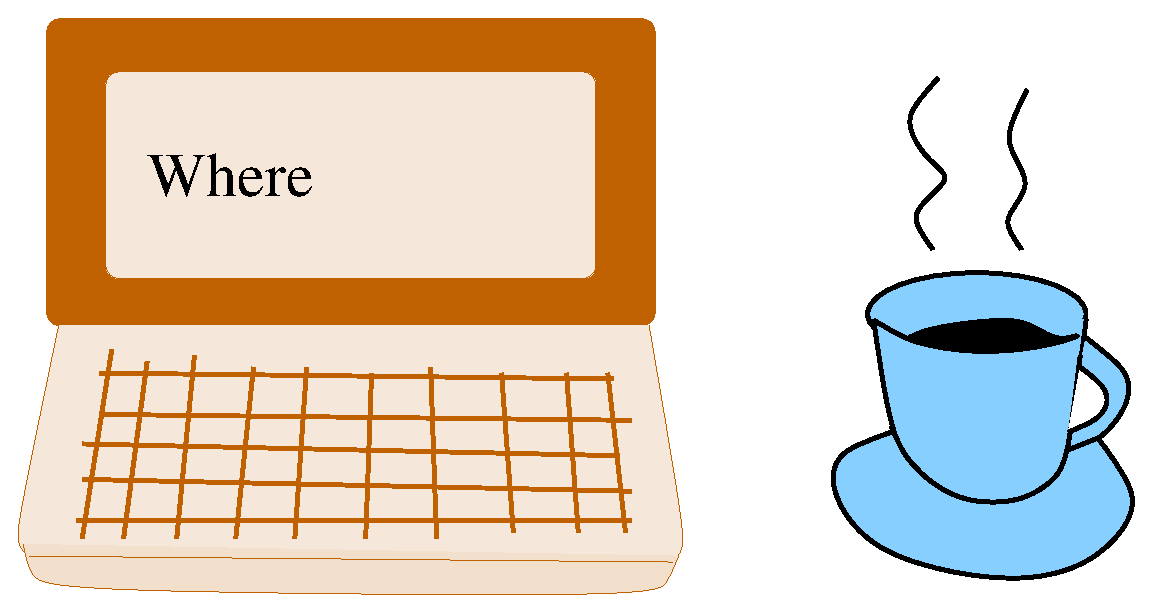
\includegraphics[width=0.95\textwidth]{figure/where.eps}
  \end{columns}
\end{frame}


\begin{frame}{Retroreflektorer}
  \begin{tabular}{cl}
    &  \\
    \raisebox{-.5\height}{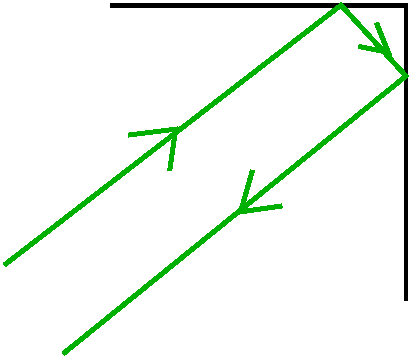
\includegraphics[width=0.2\textwidth]{figure/laser.eps}} & 
    \begin{minipage}[t]{0.6\columnwidth}Lyset reflekteres i samme retning som det kom fra \end{minipage}\\
    &  \\     
    \raisebox{-.5\height}{\includegraphics[width=0.2\textwidth]{figure/plotkin_-_beacon_explorer_a2.jpg}} & 
    \begin{minipage}[t]{0.6\columnwidth}Første satellitt med retroreflektorer, Beacon Explorer B, 1964. Henry Plotkin undersøker reflektorene.\end{minipage}\\
  \end{tabular}
\end{frame}


\begin{frame}{LAser GEOdynamics Satellite}
  \begin{columns}
    \column{0.6\textwidth}
      \begin{itemize}
        \item LAGEOS-1, 1976 (USA)
        \item LAGEOS-2, 1992 (Italia)
        \item Vekt: 400 kg
        \item Omløpstid: 220 min
        \item Høyde: 5800 km
        \item Diameter: 60 cm
        \item Levetid: 8.4 mill år. Inneholder en tidskapsel. 
      \end{itemize}
    \column{0.3\textwidth}
      \begin{figure}
        \includegraphics[width=0.7\textwidth]{figure/lageos_1.jpg} \caption{Photo: NASA}
      \end{figure}
  \end{columns}
\end{frame}


\begin{frame}{Stasjonsnettverk}
  \begin{figure}
    \includegraphics[width=0.9\textwidth]{figure/slrmap.png}\caption{Grafikk: NASA}
  \end{figure}
\end{frame}


\begin{frame}{Ny Ålesund}
  \framesubtitle{SLR ferdigstilles i 2024, bygges av NASA}
  \begin{figure}
    \includegraphics[width=0.9\textwidth]{figure/PAB_jordobservatoriet.jpg}\caption{Foto: Per Anders Bjørklund}
  \end{figure}
\end{frame}


\begin{frame}{Banen til LAGEOS-1}
  \begin{figure}
    \includegraphics[width=0.9\textwidth]{figure/orbit_l1_4h.png}\caption{Bare 5 stasjoner målte mot Lageos1 i første omløp 1. oktober 2019. Banen er beregnet med {\it Where}.}
  \end{figure}
\end{frame}


\begin{frame}{Banen til LAGEOS-1}
  \begin{figure}
    \includegraphics[width=0.9\textwidth]{figure/orbit_l1_week.png}\caption{26 stasjoner målte mot Lageos1 i perioden 1. - 7. oktober 2019. Banen er beregnet med {\it Where}.}
  \end{figure}
\end{frame}


\begin{frame}{ITRF}
\framesubtitle{International Terrestrial Reference Frame}
  \begin{description}
    \item[Hvorfor?] For å kunne måle platetektonikk, havnivå masseforflytninger etc. i referanse til noe
    \item[Hvordan?] Laget ved hjelp av fire geodetiske teknikker GPS, VLBI, SLR og DORIS
    \item[Når?] Må oppdateres jevnlig, fordi vi har nye modeller, nytt måleutstyr, og fordi jorda forandrer seg
    \item[Sist gang:] ITRF2014
    \item[Neste gang:] ITRF2020
  \end{description}
\end{frame}


\begin{frame}{Referanserammen}
  \begin{columns}
    \column{0.22\textwidth}
      \vspace{0.9cm}
      \begin{figure}
        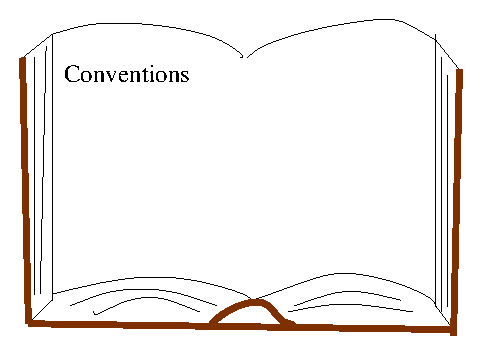
\includegraphics[width=0.95\textwidth]{figure/book.eps}\caption{Regelboken}
      \end{figure}
    \column{0.08\textwidth}\\ \ \\ \ \\ \ \\ \ \\ 
      +  
    \column{0.22\textwidth}
      \begin{figure}
        \includegraphics[width=0.95\textwidth]{figure/jordklode.eps}\caption{Observasjoner}
      \end{figure}
    \column{0.08\textwidth}\\ \ \\ \ \\ \ \\ \ \\
      =
    \column{0.26\textwidth}
      \\ \ \\ 
      \begin{figure}
        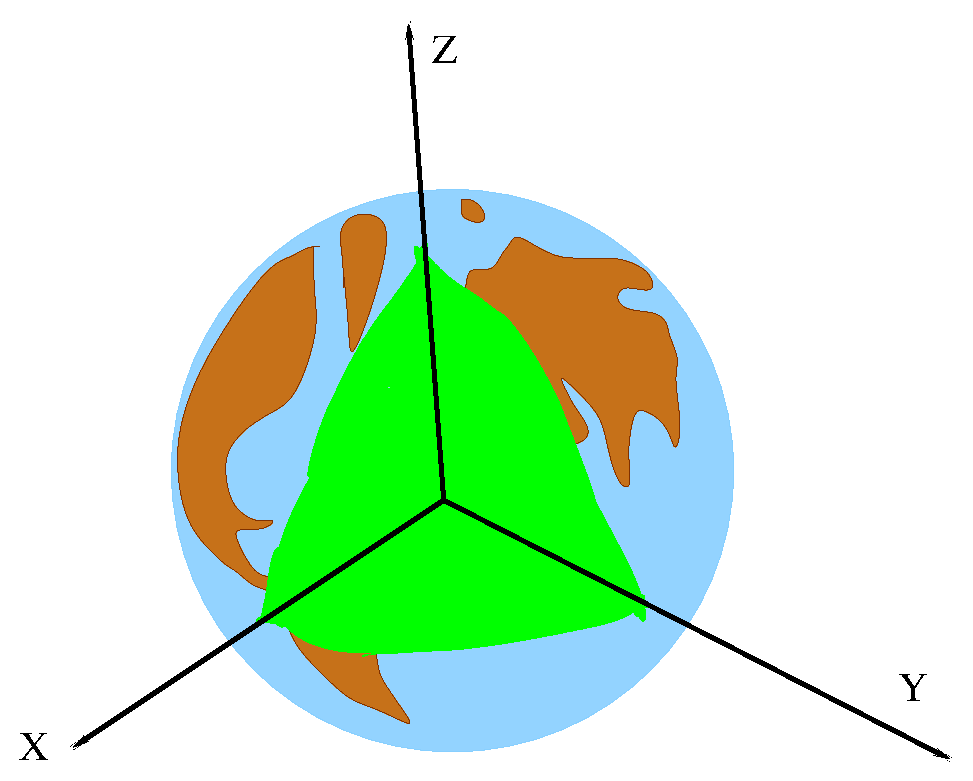
\includegraphics[width=0.97\textwidth]{figure/referanseramme.eps}\caption{Referanserammen}
      \end{figure}
  \end{columns}
\end{frame}


\begin{frame}{Jordrotasjonsparametre}
  \begin{center}
    \begin{figure}
      \includegraphics[width=0.15\textwidth]{figure/eop_parameters.png}
    \end{figure}

  \begin{figure}
    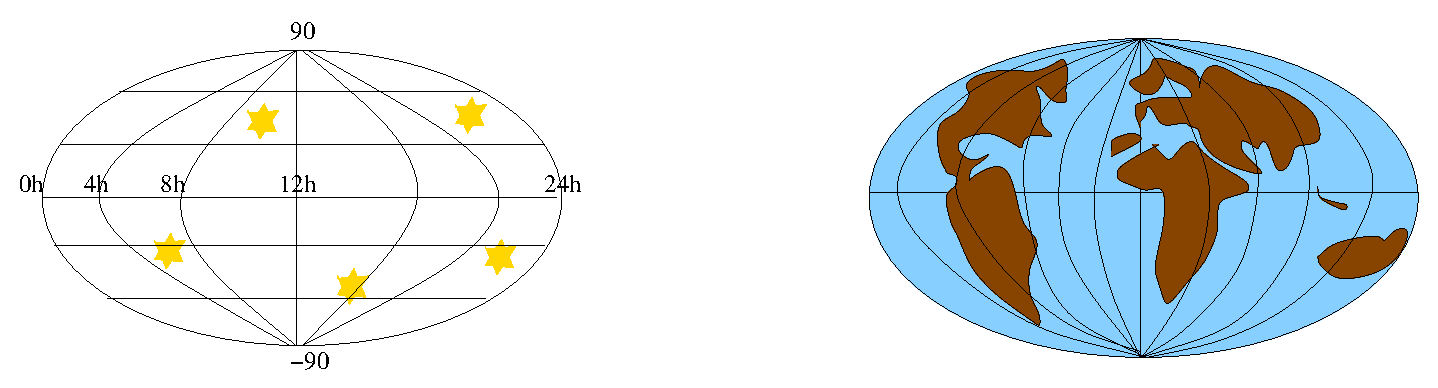
\includegraphics[width=0.8\textwidth]{figure/eop.eps}\caption{Hvordan jordfast system er rotert i forhold til himmelfast system.}
  \end{figure}
  \end{center}
\end{frame}


\begin{frame}{Verdikjeden for SLR}
\framesubtitle{(og hvor Kartverket vil være med og bidra i fremtiden)}
  \begin{tabular}{clc}
    &  \\
    \fbox{40+ stasjoner med SLR} & \includegraphics[width=0.08\textwidth]{figure/pil_horisontal.eps}  & \fbox{
          \includegraphics[width=0.1\textwidth]{figure/kartverket.png}}\\

    
\includegraphics[width=0.015\textwidth]{figure/pil.eps} && \\

    \fbox{2 datasentre i USA/Tyskland} && \\

    
\includegraphics[width=0.015\textwidth]{figure/pil.eps} && \\
    \fbox{7 analysesentre} & \includegraphics[width=0.08\textwidth]{figure/pil_horisontal.eps} &  \fbox{
          \includegraphics[width=0.1\textwidth]{figure/kartverket.png}}\\

    
\includegraphics[width=0.015\textwidth]{figure/pil.eps} && \\
    \fbox{2 kombinasjonssentre i USA/Italia} & &\\
  \end{tabular}
\end{frame}


\begin{frame}{Verdikjeden for referanserammen}
\framesubtitle{International Earth Rotation and Reference Systems Service (IERS) koordinerer arbeidet}
  \begin{tabular}{clc}
    &  \\
    \fbox{VLBI + SLR + GNSS + DORIS + Local Ties} \\

    
\includegraphics[width=0.015\textwidth]{figure/pil.eps} \\

    \fbox{Kombinasjon i Tyskland/Frankrike/USA} \\

    
\includegraphics[width=0.015\textwidth]{figure/pil.eps} \\

    \fbox{ITRF: International Terrestrial Reference Frame}

  \end{tabular}
\end{frame}


\begin{frame}{Korreksjoner}
  \begin{itemize}
    \item Betyr ikke at målingen er «feil»
    \item I SLR måler vi gangtiden til signalet, ikke faktisk avstand
    \item Forsinkelse av signalet gjennom atmosfæren utgjør 3-4 meter
    \item Signalet reflekteres ikke i sentrum av satellitten
    \item Stasjonsforflytning: Tidekrefter etc.
  \end{itemize}
\end{frame}


\begin{frame}{Baneberegning}
  \begin{itemize}
    \item Analysesentrene beregner sine egne baner
    \item Iterativ prosess, numerisk integrasjon
    \item Må ta hensyn til alle krefter som virker på satellitten
    \item Minste kvadraters metode tilpasning til målingene
    \item Bruker banen som en «fast referanse i rommet», regner ut korreksjoner for stasjonsposisjonene etterpå
  \end{itemize}
\end{frame}


\begin{frame}{Where}
  \framesubtitle{Vår programvare for geodetisk analyse}
  \begin{itemize}
    \item Utvikles ved Kartverket
    \item Skrives i Python
    \item Testleveranser til International VLBI Service pågår
    \item Plan om testleveranser også til International Laser Ranging Service i løpet av 2020
    \item Har som målsetning å bli analysesenter for VLBI og SLR
  \end{itemize}
  \begin{center}
    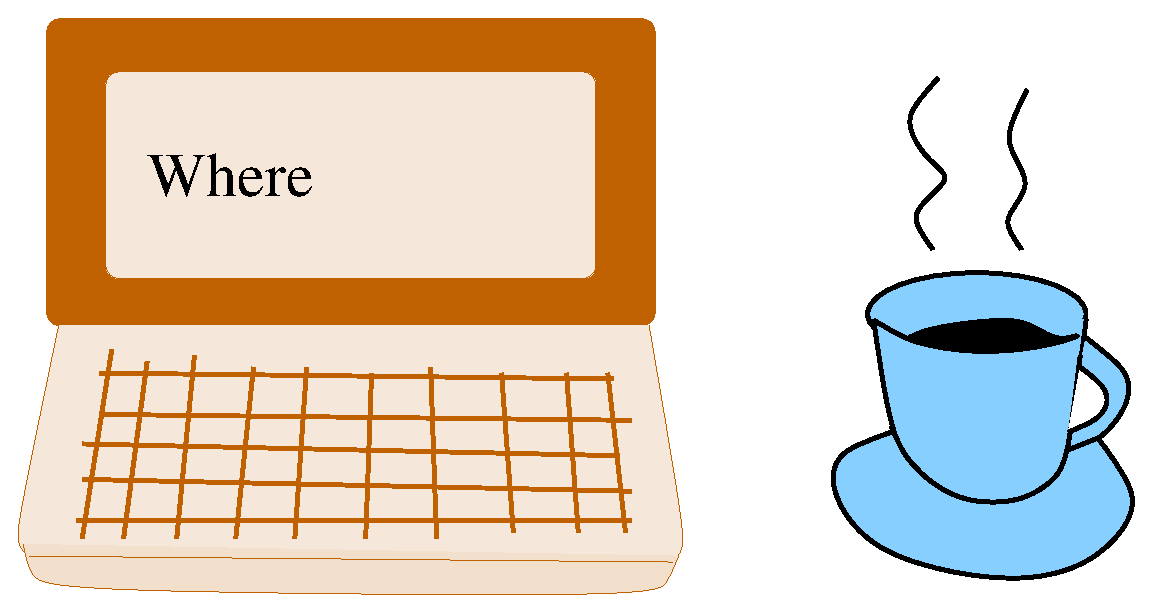
\includegraphics[width=0.3\textwidth]{figure/where.eps}
  \end{center}
\end{frame}

\end{document}
}
      \end{block}
    \end{column}
    \begin{column}{.22\textwidth}
      \includegraphics[width=\textwidth]{figure/gnss}
      \raisebox{0.3cm}{\kern-5cm\color{white}\tiny
        PHOTO: ESA -- J. HUART}
      \vskip-1ex
      \begin{block}{GNSS}
        \vskip-3ex
        \parbox[t][\techheight]{\linewidth}{Global Navigation Satellite Systems (GNSS) are networks of satellites used to accurately calculate positions on
Earth. Such systems include the American GPS, the Russian GLONASS and the European Galileo-system. They all work by
measuring the time a signal takes from the satellites to a receiver and calculating distances based on these.

\endinput
}
      \end{block}
    \end{column}
    \begin{column}{.22\textwidth}
      \includegraphics[width=\textwidth]{figure/doris}
      \raisebox{0.3cm}{\kern-8.3cm\color{white}\tiny
        PHOTO: ESA -- DENNMAN PRODUCTIONS}
      \vskip-1ex
      \begin{block}{DORIS}
        \vskip-3ex
        \parbox[t][\techheight]{\linewidth}{Doppler Orbitography and Radiopositioning Integrated by Satellite (DORIS) is a
system consisting of a network of ground-based beacons emitting signals that are
picked up by satellites as they fly by. Satellite orbits and beacon positions
can be calculated based on the Doppler effect, the frequency shift of the beacon
signal caused by the satellite movement.

\endinput
}
      \end{block}
    \end{column}
  \end{columns}
  
  \vspace*{1cm}

  \begin{columns}
    \begin{column}[t]{.47\textwidth}
      \begin{block}{Where}
        \begin{multicols}{2}
          \documentclass[12pt, english]{beamer}

% Packages
\usepackage{xcolor}
\usepackage{eulervm}
\usepackage[utf8]{inputenc}

% Theme
\mode<presentation>
{
  \usetheme{Honefoss}
  \setbeamertemplate{blocks}[rounded]
}

\newcommand{\comment}[1]{{\slshape\color{kvred}#1}}

\title{Where}
\subtitle{A Geodetic Software}
\author{Ingrid Fausk, Michael Dähnn, Ann-Silje Kirkvik}
\date{April 6, 2019}

\begin{document}
\frame[plain]{\titlepage}

\begin{frame}{Where Timeline}
  \begin{itemize}
    \item 2015: Start
    \item 2018: First release as an open source project on GitHub
    \item 2019: Two proposed IVS analysis centers with Where: 
       \begin{itemize}
         \item Kartverket, Norway
         \item Instituto Geográfico Nacional, Spain
       \end{itemize}
    \item 2020: IVS Analysis centers with Where?
    \item 2022: ILRS Analysis center with Where?
  \end{itemize}
\end{frame}

\begin{frame}{Live Demo of Where}
  \begin{itemize}
    \item Running \emph{Where}
    \item Running \emph{There}, a companion tool for visualizing results
    \item Status, discussion
    \item Bugs...
  \end{itemize}
  \begin{figure}
    \begin{flushleft}
      \includegraphics[width=2.5cm]{bug.jpg}
    \end{flushleft}
  \end{figure}     
\end{frame}

\begin{frame}{The Technical Stuff}

The \textbf{Where} software is mainly being written in \emph{Python}

  \begin{itemize}
    \item Cross-platform: Runs on Linux, Mac, Windows
    \item Solid, flexible and fast libraries like \texttt{numpy}, \texttt{astropy}, \texttt{matplotlib} and \texttt{scipy} are available
    \item We use a \textbf{HDF5}-based format for internal data storage
    \item \emph{Python} has effective interfaces to \emph{C} and \emph{Fortran} code, and we use the \textbf{SOFA} and \textbf{IERS} software libraries directly
    \item Orbit integrator using \emph{Cowell} method written in \emph{Python}. 
  \end{itemize}
\end{frame}

\end{document}

        \end{multicols}
      \end{block}

      \vspace*{3cm}
  
      \begin{figure}
        \includegraphics[width=0.7\textwidth]{figure/architecture}
        \caption{The software architecture.}
      \end{figure}
    \end{column}
      
    \begin{column}[t]{.47\textwidth}
      \begin{block}{Examples}
        \begin{multicols}{2}
          Let us look at a few examples on how to run the Where software. One of our
guiding principles is that the software should be as easy to use as possible.

{\bfseries A VLBI analysis}

To start a VLBI analysis, we simply need to provide the date we want to analyse:

\texttt{> where 2016 6 22 --vlbi}

Doing this will show the default configuration for VLBI analyses, including
options like which models to run, which ephemerides (positions for planets etc)
to use and which output to create. All of these options can be changed, or we
can accept the defaults and run the analysis.

As the model runs, all intermediary calculations are stored, allowing us to
later look at data at each step. For instance can we compare raw observation
numbers with calculated results, or look at the residuals before or after
estimation. The simplest way to do this is to use the There GUI-companion:

\texttt{> there}

\includegraphics[width=\linewidth]{figure/vlbi_20160622_nyales20}

{\itshape Residuals based on models (no estimation) from a VLBI analysis for the
  station at Ny-{\AA}lesund, Norway. Colors indicate the other station in the
  baseline.}

After a model run, we can also explore the data interactively. In practice, this
means that we get access to the datasets and can use the Python datastack to
manipulate them:

\texttt{> where 2016 6 22 --interactive}

\begin{verbatim}
Available datasets:
    v0, vlbi_calculate_XA_1
    v1, vlbi_calculate_XA_2
    v2, vlbi_edit_data_XA_0
    [...]

In [1]:  v1.residual
array([ 0.47276345, -0.05613388,
       -0.50012711, ...,  0.05031952,
       -0.00214976,  0.04906757])

In [2]: v1.unique('station')
['BADARY', 'MEDICINA', 'NOTO',
 'NYALES20', 'SVETLOE', 'WETTZELL',
 'YEBES40M', 'ZELENCHK']
\end{verbatim}

The final output of the analysis can be stored in many different formats. Sinex
is typically used when sharing analysis with others. However, one interesting
output format Where supports is Jupyter Notebooks. These allow us to for
instance run each model independently, and easily create live demonstrations of
the software highlighting particular parts of the analysis.

{\bfseries A GPS analysis}

Doing a GPS analysis is done in the same way as the VLBI analysis. We only need
to specify a different technique:

\texttt{> where 2016 6 22 --gnss}

The technique is specified as \texttt{--gnss} because Where will support
analyses of several of the systems, including GLONASS and Galileo, in addition
to GPS. Running Where like this will again bring up all the default options. For
GNSS these options will now include how to handle satellite orbits and which
stations to analyse.


\endinput

        \end{multicols}
      \end{block}

      \begin{block}{Future}
        \begin{multicols}{2}
          At the moment we work on challenges connected to the combination of VLBI and SLR epoch by epoch. One important issue in this respect will be how we tie the VLBI and SLR network together. For instance, it will be important that the networks are closely connected at an early stage (during epoch by epoch processing with UD Kalman filter) so that the techniques may fully complement each other, before we truncate the state vector and its variance-covariance matrix for the accumulated combination solution. To what extent will the Earth Rotation Parameters, shared by both techniques, connect the different networks and, alternatively, how will we use local ties? Shall we use all available local ties, or only the most reliable?

The output of each data set will be a state vector consisting of global (station coordinates) and stochastic parameters (clock, troposphere) at the last epoch of the data set. Although no approximations regarding correlations have been made at this stage, the solution's a posteriori variance-covariance matrix does not contain all available information on parameter correlations. If we use only this limited information (state and covariance at last epoch), as we intend to due to practical reasons (see Combination), it is possible that we during day by day combination have to involve Helmert transformations to describe the weaknesses of daily solutions.       

In the future we will include GNSS and DORIS in our processing chain, which we anticipate will require the introduction of new parameter types to achieve intra-technique consistency.    


\endinput

        \end{multicols}
      \end{block}
    \end{column}
  \end{columns}
\end{frame}
\end{document}

% Keep getting a ! LaTeX Error: There's no line here to end.
% Not sure why ... the output looks ok
